%!TEX root = paper.tex
In this section we discuss the simulations we ran in order to verify our extension's ability to enable PAC search over BitTorrent. In the simulations we model complex node behaviour that is not accounted for in our models and analysis so far. Each of our simulations creates a BitTorrent network of 5 million nodes, each node operating independently of each other. We simulate a single torrent in the network and analyse the queries, replication and participation over time. Each simulation is comprised of multiple trials, trials are repeated until the minimum number have been run or the confidence level of the recorded statistics is 5\%, which ever is greater. For each simulation we apply a PAC search using a query size of $z=100$. Until now we have assumed that network churn removes a constant proportion of nodes from the network every hour. In \cite{Qiu2004,Guo2007} a fluid model of BitTorrent networks is created that instead describes churn as a function of each individual node's time spent in the network, a combination of time spent downloading the torrent and time spent seeding it. In this model the amount of time a node is willing to seed a torrent for is assumed to be exponentially distributed with mean $\tfrac{1}{\gamma}$. In order to implement this, we have each node sample from an exponential distribution with $\gamma=0.01\dot{6}$ in order to determine how long to seed the torrent for. The amount of time spent downloading the torrent is more complicated; the maximum amount of time a node is willing to wait for a download to complete is exponentially distributed with mean $\tfrac{1}{\theta}$. The actual time spent downloading is determined by the node's available download bandwidth and the amount of upload bandwidth available from participating nodes. We implement this by assuming that each node's bandwidth allows for a maximum of 10\% of the torrent file to be downloaded every hour and 1\% of the torrent file to be uploaded. We then have each node sample from an exponential distribution with mean $\theta=0.025$ in order to determine how long they are willing to wait. If there are enough participating nodes that a node can complete a download before aborting then the node seeds the torrent for the randomly sampled time period described above. If a node aborts a download or finishes seeding, then the node leaves the network. In order to keep network size a constant 5 million, when a node leaves, we add a fresh node to the network to compensate. This more complex model of churn allows us to verify our extension under a more realistic setting. We model and observe a single torrent in the network for a maximum of 450 hours. Not every node participates in the observed torrent. Nodes that do not participate still exhibit the behaviours outlined above but they make no PAC queries. Instead they simply progress through their downloading and seeding phases, responding to any PAC queries made of them, before leaving the network.

Using this model for churn we ran simulations of torrents with constant numbers of participating nodes, i.e. whenever a participating node left the network it was immediately replaced by another, new, participating node. We ran three such simulations: one for a torrent with a constant 1000 node participation; one with 100; and one with 10. These numbers cover the range of constant participation observed by the authors in \cite{Gummadi2003}, who noted that a significant number of torrents over 40 weeks old displayed a constant level of participation. With constant participation the amount of time it took each node to download the torrent was almost equal across all nodes. This meant that we observed a close to constant query rate. Figure~\ref{fig:probability_constant_churn} shows the probability of a successful query over time for the three simulations. As expected from our previous analysis, with a constant query rate we observe a steady probability. When the participation is set to 10 nodes we observe an average probability of a successful query of 14.26\%, this might seem low, but each joining node is running an average of only 8 queries before success. This is in-line with our previous analysis and shows that even if only 10 out of 5 million nodes own a torrent our extension enables that torrent's discovery. For greater levels of participation the probability of successful query is higher and therefore the torrent is even easier to find. When 1000 nodes participate, the average probability of finding the torrent after a single query to 100 nodes is 87\%.

\begin{figure}[t]
    \centering
    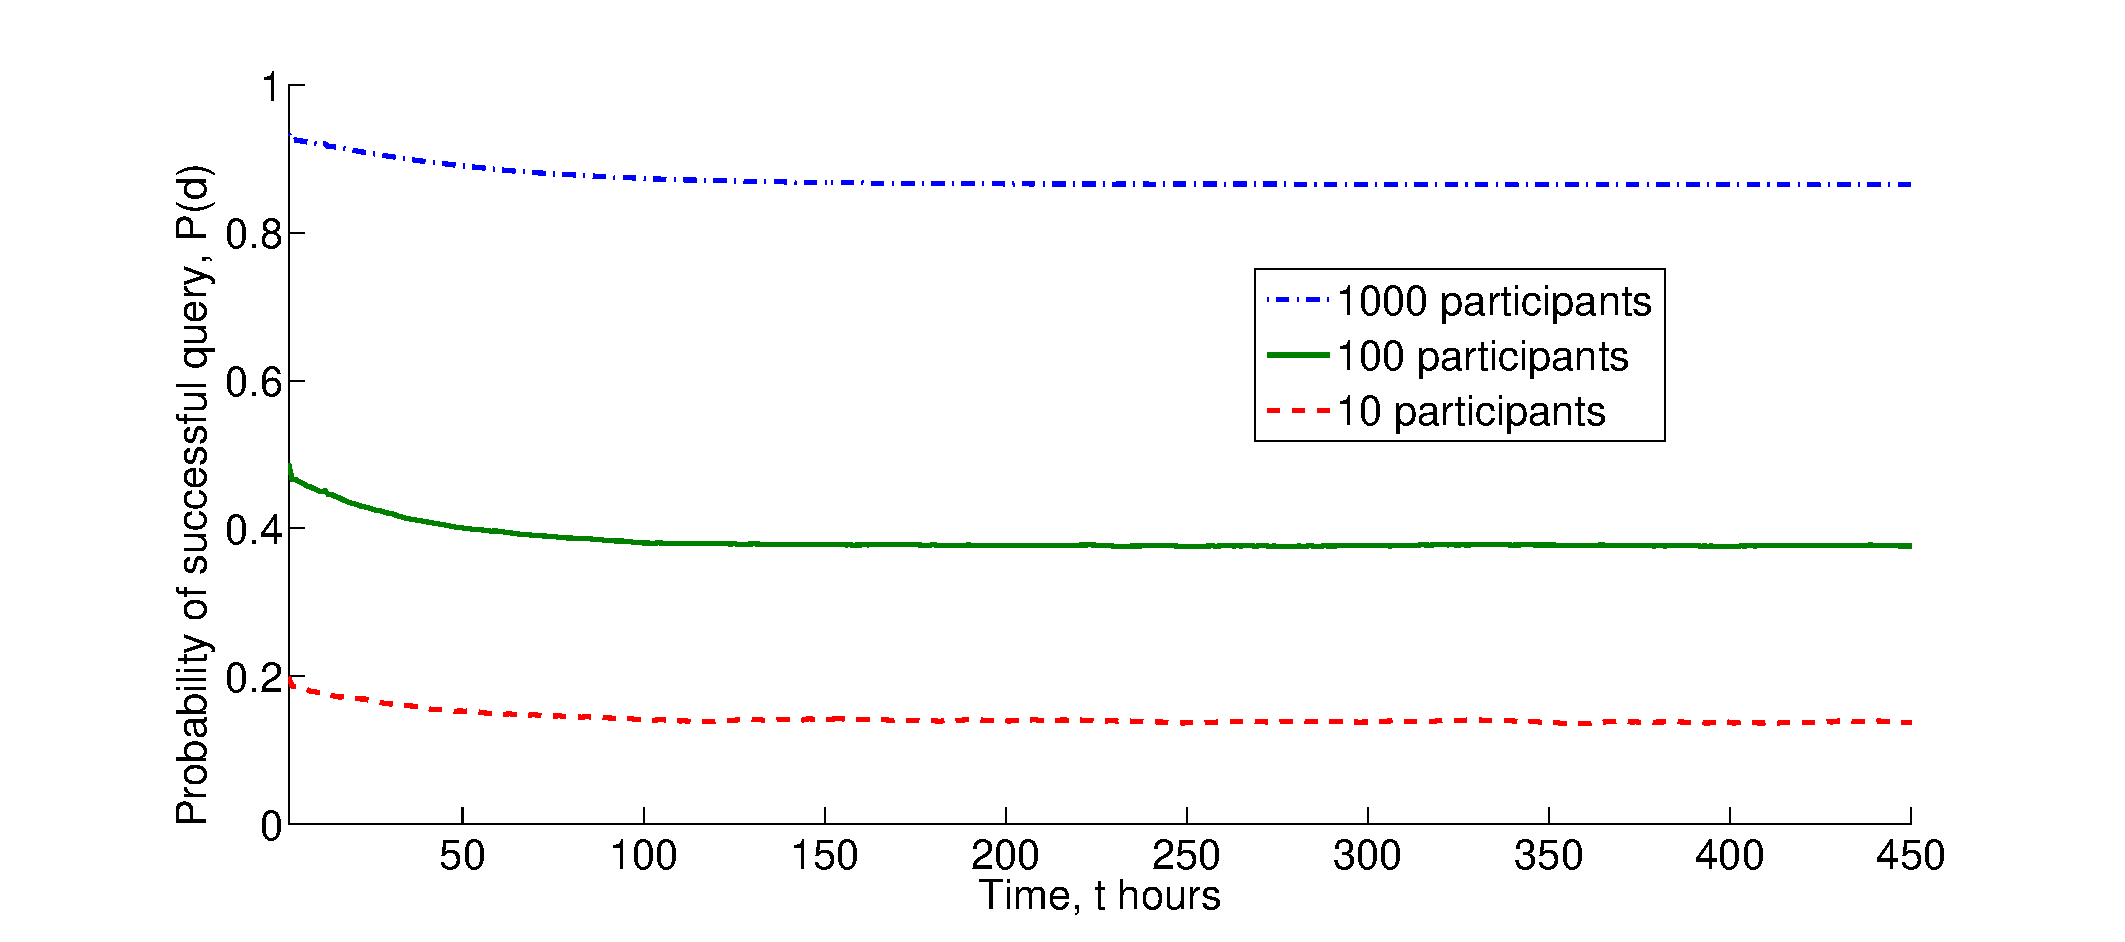
\includegraphics[width=0.5\textwidth]{Images/ProbabilityConstantChurn.eps}
    \caption{The probability, $P(d_i)$, of a successful query over time for three different levels of constant torrent participation.}
    \label{fig:probability_constant_churn}
\end{figure}

Our next set of simulations explore what happens if a fixed number of nodes participate in a torrent but no additional queries are made for it. In this situation we define a fixed number of nodes that remain in the seeding state for the duration of the simulation. No nodes search for the torrent and so the replication decreases with network churn. Figure~\ref{fig:probability_constant_static} shows the probability of a successful query for torrents with fixed participation levels of 1000, 100, and 10 nodes. We observe that the probability declines at an almost linear rate, dropping between 11.55 and 28.51 percentage points over the 450 hours of the simulation. We conclude that if a torrent's participating nodes remain in the network then our extension is reasonably resilient to churn before any steps have been made to mitigate it. This is because each participating node will have replicated tracking data that will never become incorrect. If these nodes wished to stabilise the probability of discovering their torrents then they could make dummy requests to mitigate the loss of replication due to network churn. For participation levels of 1000, 100, and 10 on average as few as 181, 46, and 15 dummy requests per hour would have to be made respectively.

\begin{figure}[t]
    \centering
    \includegraphics[width=0.5\textwidth]{Images/ProbabilityConstantStatic.eps}
    \caption{The probability, $P(d_i)$, of a successful query over time for three different levels of fixed torrent participation.}
    \label{fig:probability_constant_static}
\end{figure}

Our next simulations use the fluid model from \cite{Qiu2004,Guo2007} to model not only the network churn but also query rate over time. Our analysis so far has assumed a query rate at or near a constant value but we cannot expect that torrents will always exhibit such constant popularity. In the fluid model, query rate is determined using the node arrival time; the amount of time that passes before a node first starts to participate in the torrent. Node arrival time is exponentially distributed with mean $\tfrac{1}{\lambda}$. In our simulations a number of nodes are chosen to participate in the torrent, each node samples form an exponential distribution with mean $\lambda=0.0\dot{3}$. This tells the node how many hours to wait before initiating a PAC search. We simulate three types of torrent; torrents whose participation peaks at 10,000 simultaneous nodes; torrents with a peak at 1000 nodes; and torrents with peaks at 100 nodes. These numbers broadly cover the range of participation we observed in our measurement study. We omit torrents with a participation peak of one node because there is no query rate to simulate over time. Such a torrent, and any torrents with similarly small participation, will {\emph have} to have nodes issues dummy requests in order to make the torrent discoverable, as discussed in Section~\ref{sec:extension}. Figure~\ref{fig:probability_exp_standard} shows the probability of a successful query over time during these three simulations. As expected, if a torrent has a higher participation then it's tracking data will have higher replication and so the probability of success will be greater. Interestingly, under this model of query rate the probability of successful query peaks with the participation and so is greatest when the most queries are being performed. For this reason the average probability of a successful query is 99.06\% for torrents that peak at 10,000 nodes, 78.61\% for torrents that peak at 1000, and 25.68\% for torrents that peak at 100. This is despite seemingly long tail of lower probabilities for each curve. The average number of queries required before success was 6 for the worst performing curve, meaning that even if a node is searching for a torrent whose participation never exceeds 100 nodes in 5 million, only 6 queries are expected to be required before success.

\begin{figure}[t]
    \centering
    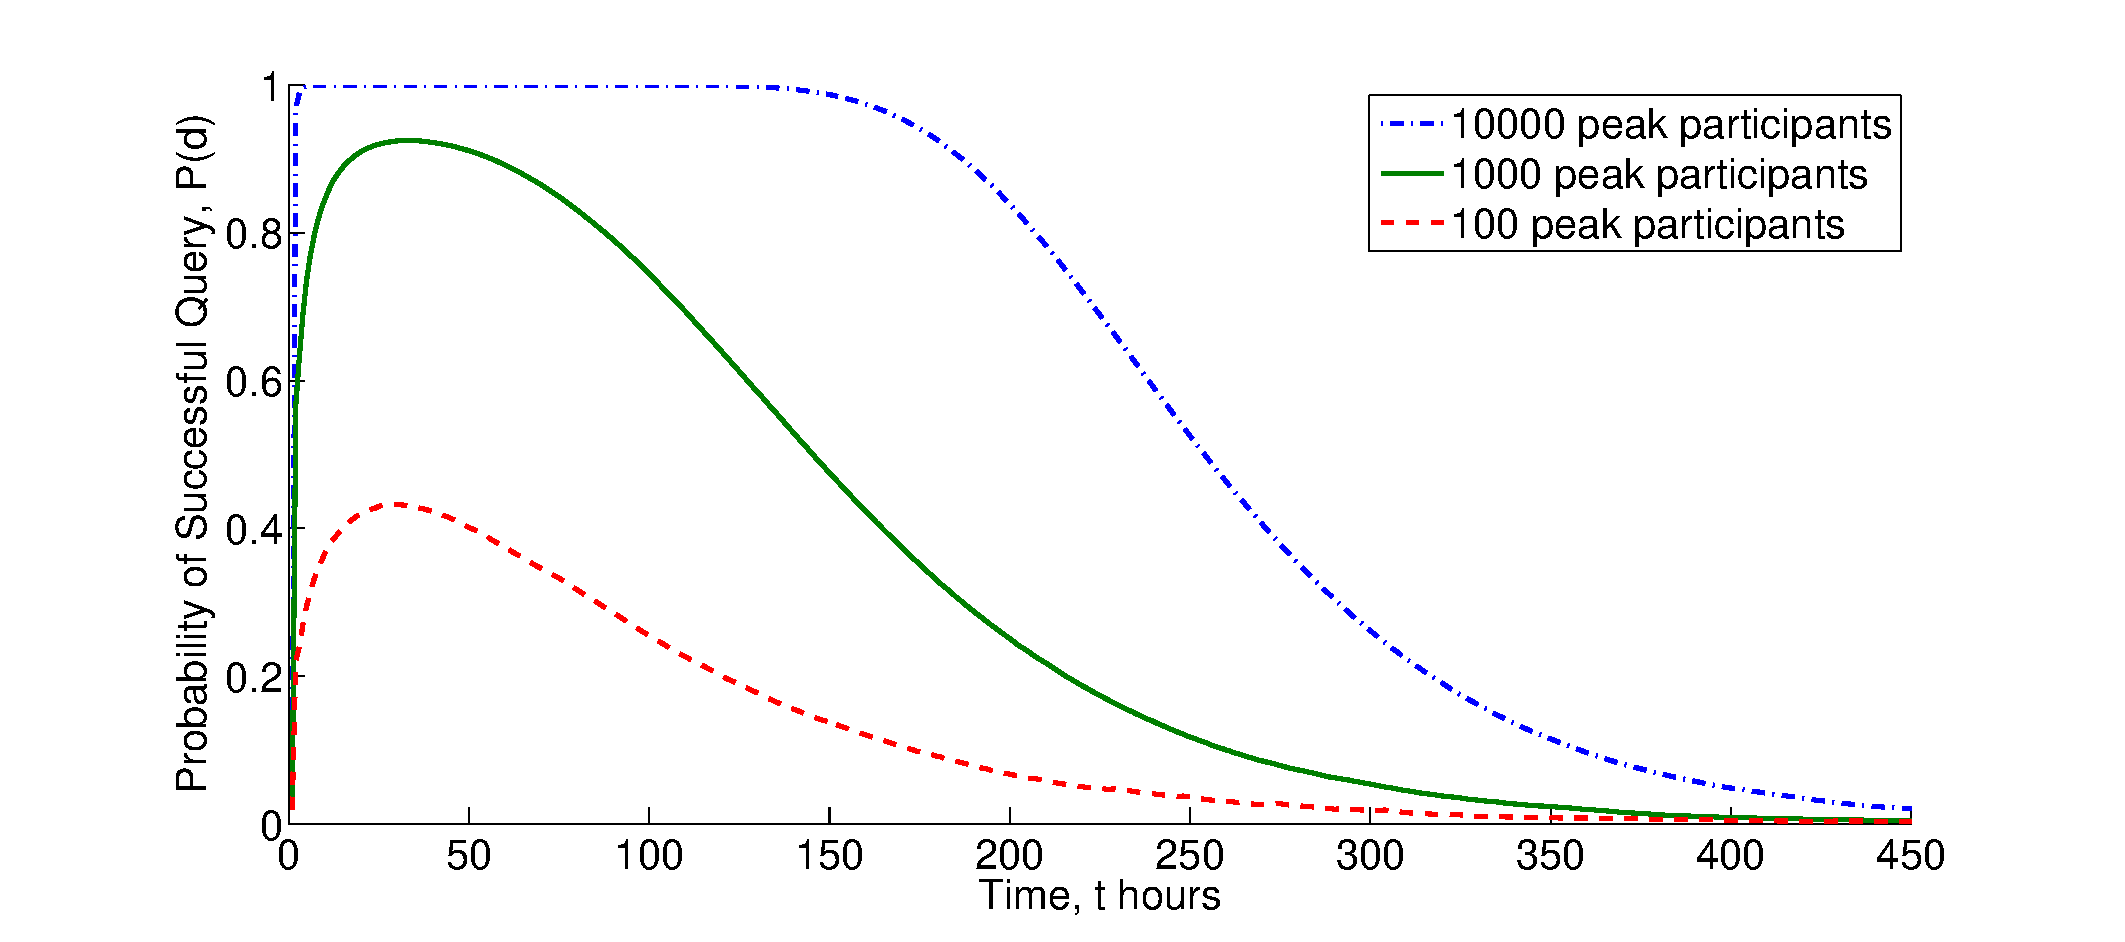
\includegraphics[width=0.5\textwidth]{Images/ProbabilityExpStandard.eps}
    \caption{The probability, $P(d_i)$, of a successful query over time for three different levels of peak participation under fluid modelled query rates.}
    \label{fig:probability_exp_standard}
\end{figure}